\section{Verbesserung von Strukturvorhersagen}
Im folgenden sind mehrere Faktoren aufgeführt, die zur Optimierung der Strukturvorhersage bzw. die Vollständigkeit der Strukturvorhersage zeigen. Weiterhin kommt die komparative Analyse von RNA-Strukturen mit hinein, die aufgrund der evolutionär wichtigen Struktur-Funktions-Beziehung wichtige Aussagen über Strukturen geben können. 

\subsection{Energieparameter}
Das Turner-Modell führte zur Erzeugung von fast 100 Parametern, die zur Ermittlung der thermodynamischen Energie eines RNA-Moleküls relevant ist zu bestimmen. \\
Andronescu et al. (2007) \footnote{Andronescu,M; Condon,A; Hoos, H; Mathews, D; Murphy, KP(2007): Efficient parameter estimation for RNA secondary structure prediction. Bioinformatics. 2007;23(13):19-28.} entwickelten eine "Constraint Generation"-Methode bei der die Schätzung der Energieparameter auf Grundlage von bekannten thermodynamischen Datenbanken errechnet werden. \\
Hierbei werden zunächst die Energiewerte zur Berechnung der besten Struktur genutzt und durch ein Optimierungsproblem über mehrere Iterationsschritte verbessert, so dass die Energie minimal wird.

\subsection{Dangling ends}
\begin{itemize}
\item die ungepaarten Basen am Ende eines Stacks, werden als Dangling Ends bezeichnet.
\item aufgrund ihre Instabilität als Einzelsträngige Teilsequenz sind diese Bereiche recht flexibel und können auf benachbarte Basen(-paare) umspringen um einen stabileren Zustand zu erreichen.
\item 3'-Dangling Ends sind stabiler als 5'-Dangling Ends
\item Dangling Ends werden als Ursache für coaxial Stacking diskutiert (Verdrehen und Rotation bestimmter Stacks zu anderen in einer Struktur)
\item in der Berechnung werden diese Dangling Ends ebenfalls mit einem Strafbetrag verrechnet (Dangling-End-Parameter im Turner-Parameter-Modell)
\end{itemize}

\subsection{Training der Energieparameter}
Andronescu:
\begin{itemize}
	\item Set von bekannten Strukturen aus Datenbank
	\item Turner-Parameter (thermodynamische Parameter)
	\item Strukturvohersage: perturbieren (verändern, stören) der Parameter, versuche den Abstand zwischen vorhergesagten und richtigen Strukturen zu minimieren
	\item update Parameter
\end{itemize}

\textbf{Problem:} Training nur auf bekannten Daten, für unbekannte Strukturen nicht immer besser

\subsection{Constraint Folding}
Man unterscheidet zwei Typen von Constraints (Beschränkungen):
\begin{itemize}
\item[Hard Constraints] Es darf keine Basenpaarung einer anderen widersprechen. Entweder eine Base i ist ungepaart oder ist nach links oder nach rechts mit einer anderen verbunden. 
\item[Soft Constraints] Ergeben sich aus den Energiescorematrizen der Strukturvorhersage mit McCaskill (oder Zuker) und zeigen die Wahrscheinlichkeit einer bestimmten positionsabhängigen Basenpaarung an
\end{itemize}

Experimentell kann durch Methoden, wie PARS (Hochdurchsatz-Sequenzierung) bestimmt werden an welchen Positionen Basenpaarung vorliegen. Hierfür wird ein bioenzymatischer Verdau durchgeführt bei dem entweder doppelsträngige Stellen oder einzelsträngige Stellen zersetzt werden.
\\\\
\textbf{RNA $\rightarrow$ Struktur (Funktion) $\rightarrow$ evolutionär konserviert (Verwandschaft)}

- es ist möglich Struktur und damit Funktion zu konservieren auch wenn die Sequenz verändert wird

\begin{itemize}
	\item konsistente Mutation: G-C $\rightarrow$ G-U
	\item kompensatorische Mutation: Mutation an C zieht Mutation an G mitsich
\end{itemize}

\underline{$\Rightarrow$ Ziel:} Zusätzliche Informationsebene durch auffinden von konsistenten und Kompensatorischen Mutationen
\\\\
$\Rightarrow$ benötigt Set von n Sequenzen, die die gleiche Struktur haben
\\\\
\underline{nun drei Möglichkeiten:}
$\rightarrow$ prinzipiell: Alignments mit Sekundärstrukturvorhersage kombinieren
\begin{enumerate}
	\item zuerst Strukturvorhersage, dann Aligenment von Strukturen (Tree Alignment)
	\item simultan alignen und Strukturen vorhersagen (Sankoff ($O(n^6)$))
	\item zuerst alignen und dann Strukturen der Alignments vorhersagen (RNA Alifold)
\end{enumerate}

\section{Konsensusstrukturvorhersage - Komparative Analyse}

In der Evolutionsbiologie geht man von einem Struktur-Funktions-Beziehung konservierter Merkmale aus. Das bedeutet: Funktional wichtige Sequenzbereiche sind in der DNA konserviert. \\
Für die RNA-Strukturvorhersage ist jedoch zu beachten, dass auch sich unterscheidende Sequenzen strukturell ähneln können und somit deren Sekundärstruktur evolutionär konserviert ist. \\
Betrachtet man nun einen Datensatz von RNA-Sequenzen kann über Alinierung der Sequenzen und/oder der Sekundärstrukturen die Ähnlichkeit dieser Sequenzen betrachtet werden. Es ist möglich, dass RNA-Moleküle mit ähnlicher bis gleicher Struktur miteinander verwandt sind. \\
$\rightarrow$ komparative Analyse:
Es gibt drei Hauptmethoden, die zur Konsensusstrukturvorhersage genutzt werden: 
\begin{itemize}
\item Funktionsvorhersage \\
\item Zuordnung von RNA-Klassen \\
\item Motivsuche
\end{itemize}

\subsection{RNAaliFold- zuerst alignen, dann falten}
$\rightarrow$ multiples Sequenzalignment (z.B. Needleman-Wunsch) \\
$\rightarrow$ generalisierte Bestimmung einer RNA-Struktur \\

\textbf{- minimiere die mittlere Energie} \\
Für RNAalifold ist ein multiples Alignment mit K Sequenzen der Länge m gegeben. Ziel ist es eine RNA-Struktur der Konsensussequenz zu finden, deren minimierte Energie sich aus der Summe aller freien Energien der K Sequenzen und dem Konservierungsgrad gleichbleibender Sequenzen zusammensetzt.\\
\\
\textbf{- Unterscheidung von Mutationen} \\
konsistente Mutationen (GC $\rightarrow$ GU) \\
und kompensatorische Mutationen (GC $\rightarrow$ UA) \\ 

Berechnung:
\begin{equation}
C(i,j)= max
\begin{cases} 
H(i,j)\\ 
I\\ 
M\\
\end{cases}
\end{equation}

$\rightarrow$  Rechne den Term, der die Konservierung beschreibt zu C(i,j) \\
$\rightarrow$ Bestrafung von Verletzung der Komplementarität\\
\begin{itemize}
	\item[Fall1:] 
	\begin{equation}
	\gammaup(i,j)= \sum 
	\begin{cases} 
	h(s_{1i},s_{2i}) + h(s_{1j},s_{2j}) \ if\ s_{1i},s_{1j}) \epsilon\ Bp \ and \ s_{2i},s_{2j} \epsilon\ Bp \\
	0 \ else\\
	\end{cases} 
	\end{equation}	
	\item [Fall2:] 
	\begin{equation} 
	C(i,j)= y * \gammaup (i,j) + x * \delta (i,j)+ mean[C(i,j)]  
	\end{equation} ;
	\begin{equation}	 
	\delta(i,j)= \sum_{S} 
	\begin{cases} 
	0 \ if\ (s_{i},s_{j}) \epsilon\ Bp \\
	0,5 \ if\ s_{i},s_{j} \epsilon\ \{-\} \\ 
	0 \ else\\
	\end{cases}
	\end{equation}
\end{itemize}

Es können so auf Wissen basierte Matrizen mit bekannten konservierten RNA-Strukturen erzeugt werden
$\rightarrow$ Ribosum: knowledge-based Score, für die Wahrscheinlichkeit in einem Basenpaar (i,j) für die Basen $s_{1i}, s_{1j}$ und $s_{2i}, s_{2j}$ \\

$\rightarrow$ Komplexität: $\Omega(n^{3}m)$ \\

Problem: Es werden nur Konsensussequenzen gefalten. Somit ist nur Allgemein eine Faltung für alle Sequenzen vorliegend. \\
Somit nur sinnvoll, wenn zum einen ein Alignment möglich ist und wenn die Sequenzen sehr ähnlich zueinander sind.

\subsection{Sankoff-Algorithmus - gleichzeitiges Alignen und Falten}

\textbf{Programm:} locarna \\

\textbf{Annahme:} Zwei Sequenzen sind sich ähnlich, wenn ihre RNA-Struktur einen stark äquivalenten Shape besitzen (len(A) = len(B) und pair(A) = pair(B)).\\

\textbf{Idee:} Finde für äquivalente Strukturen die minimale Editierdistanz  bzw. mfe \\

\textbf{Vorgehen:} Sankoff = Zuker + Needleman-Wunsch
\begin{itemize}
\item[1] Gegeben sind zwei Sequenzen A und B
\item[2] Finde äquivalente Strukturen in Sequenzen
\item[3] Erzeuge ein zu Strukturen kompatibles Alignment beider Sequenzen
\item[4] Editiere Alignment und Faltungen um minimalen Score $min(E_A + E_B + Distanz_AB)$ zu finden
\item[5] Consensussequenz und Sequenz C gegeben $\rightarrow$ gehe zu 2
\end{itemize}
\textbf{Distanzbestimmung:}
\begin{equation}
A(i,j;k,l)= min \begin{cases} 
A(i+1,j;k+1,l) + \sigma \\
A(i+1,j;k,l) + \sigma_{gap} \\
A(i,j;k+1,l) + \sigma_{gap} \\
\end{cases}
\end{equation}
\textbf{Initialisierung:}
\begin{equation}
A(i,i;k,k) = \begin{cases} \sigma \ if a_i != b_k \\ 0 \ else\end{cases}
\end{equation}
\begin{equation}
C(i,i;k,k) = \infty
\end{equation}
\begin{equation}
M(i,i;k,l) = M(i,j;k,k) = \infty
\end{equation}
Freie Energie der Sequenzen von i bis j bzw. von k bis l:
\begin{equation}
F(i,j;k,l)= min \begin{cases}
F(i+1,j,k+1,l) + A(i,j+1;k,l+1) \ (i,k \ ungepaart) \\
\\
min_{u,v}\ 
\begin{split}
C(i,u;k,v) + F(u+1,j,v+1,l) \\
+ A(u,u+1;v,v+1) + A(i,i;j,j)) \\ 
\end{split}
\ (i,k \ gepaart \ mit \ k,v)\\
\end{cases}
\end{equation}
eingeschlossene Energie zwischen dem Basenpaar (i,j) bzw. (k,l)
\begin{equation}
C(i,j;k,l)= min 
\begin{cases} 
H(i,j) + H(k,l) + A(i,j;k,l) \\ 
\\					
\displaystyle\min_{i < u < v < j \ k<x<y<l}\ 
\begin{split}
I(i,j;k,l;u,v;x,y) + C(u,v;x,y)  \\
+ A(i,u;k,x) + A(v,j;y,l)\\ 
\end{split}
\\
\\
\displaystyle\min_{i<u<j \ k<x<l}\ 
\begin{split}
M(i,u;k,x) + M^{1}(u+1,j-1;x+1,l-1) \\ 
+ A(u,u+1;x,x+1) + A(i,i+1;x,x+1) \\ 
+ A(j-1,j;l-1,l)\\ 
\end{split}
\end{cases}
\end{equation}
Energie von Mulitloops:
\begin{equation}
M(i,j;k,l) = min
\begin{cases}
M(i+1,j;k+1,l) + A(i,i+1;j,j+1) \\
\displaystyle\min_{i<u<j \ k<x<l}\ C(i,u;k,x) + A(u,j;x,l) \\
\displaystyle\min_{i<u<j \ k<x<l}\ C(i,u;k,x) + M(u+1,j;k+1,x) + A(u,u+1;x,x+1) 
\end{cases}
\end{equation}
\begin{equation}
M^1(i,j;k,l) = min
\begin{cases}
C(i,j;k,l) \\
M^1(i,j-1;k,l-1) + A(j-1,j;l-1,l)
\end{cases}
\end{equation}
$\rightarrow$ \textbf{Komplexität:} $\Omega(Zeit) = \Omega(n^6) \ ; \ \Omega(Memory) = \Omega(n^4)$ $\rightarrow$

\subsection{TREEforester - zuerst falten, dann alignen}
\begin{itemize}
\item Wie alignt man gefaltete RNA-Strukturen? \\
Nach welchen Kriterien wurde die scheinbar beste Faltung gewählt? $\rightarrow$ Tree-Editing (Bestrafung von strukturellen Mismatches)
\item Sind sie überhaupt kompatibel nach ihrer Einschränkung? (Liegen Überkreuzungen vor und sind die Grundvoraussetzungen der Struktur gleich, z.B. keine Pseudoknots) $\rightarrow$ Tree-Alignment
\item Im Falle von sich nicht kreuzenden RNA-Strukturen werden Bäume als vergleichende Datenstruktur erzeugt. Ein RNA-Baum ist ein geordneter Baum dessen Knoten einzelne Basen oder Basenpaare darstellen
\item Insgesamt können somit alle Bäume zu einem RNA-Strukturen-Wald zusammengefasst werden (RNAforester). \\
\end{itemize}
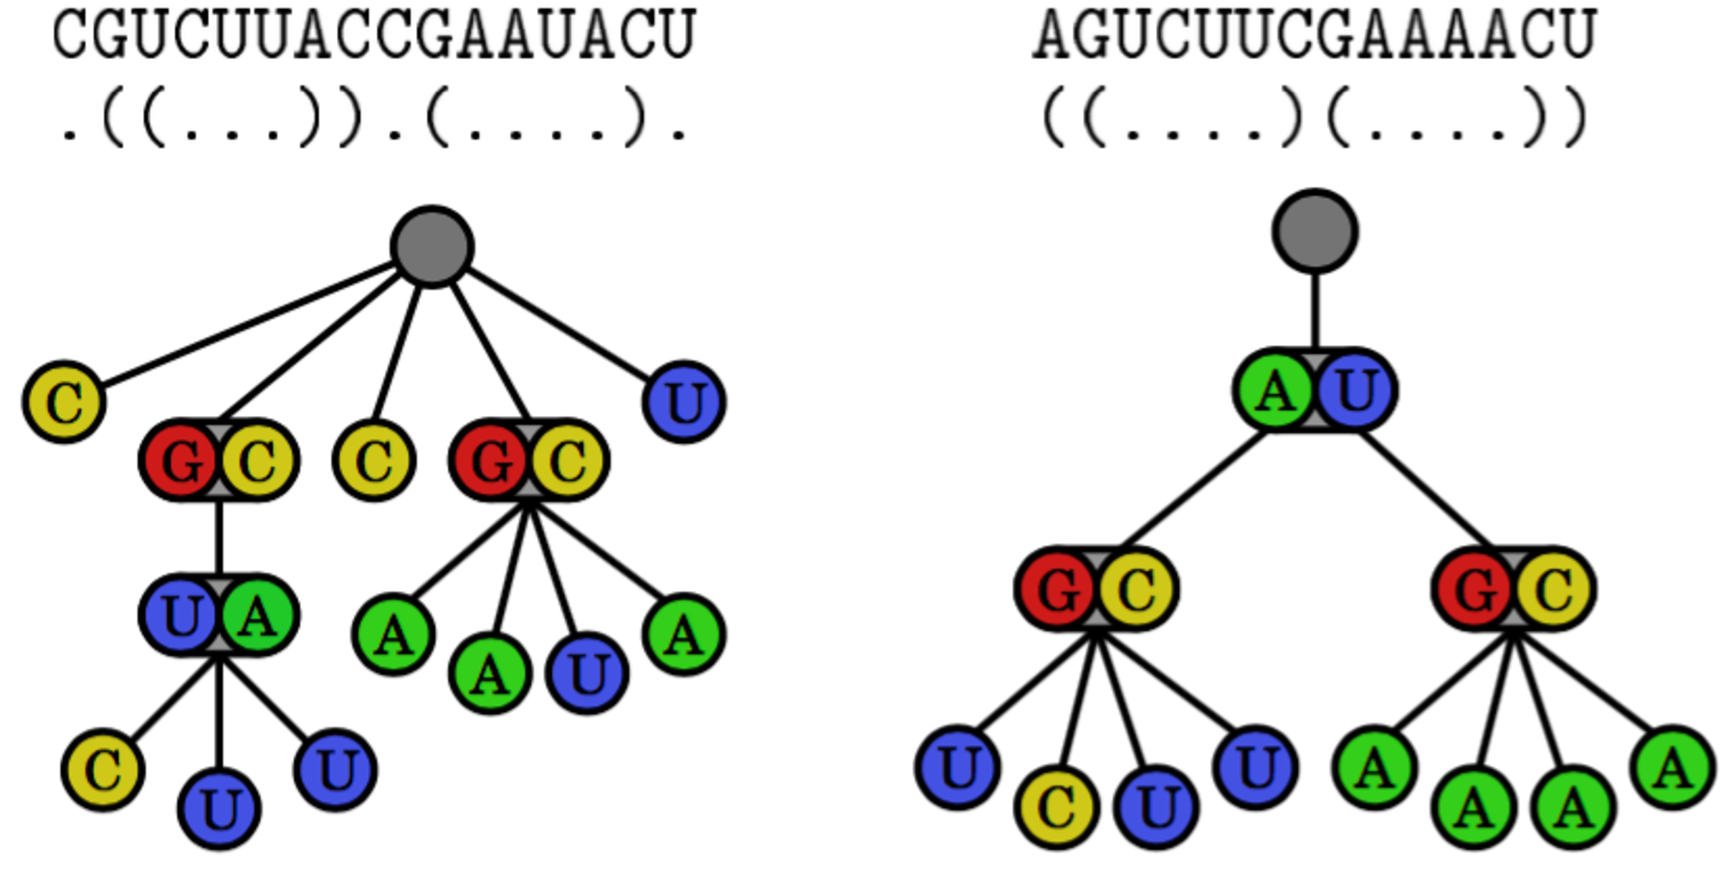
\includegraphics[scale=0.5]{lectures/160509/pix/Baeume.pdf} \\

\textbf{Tree-Editing:} wandle Baum A in Baum B um
\begin{itemize}
\item Basen umbenennen
\item Basen löschen/hinzufügen
\item Basenpaare umbenennen
\item Basenpaare hinzufügen/löschen
\end{itemize}

\textbf{Tree-Alignment:} Erzeugung eines common Super-Trees

\subsection{lokales Falten}

Vorhersagequalität nimmt mit Moleküllänge ab \\
Viele Moleküle haben keine globale Struktur aufgrund der Interaktionen in der Zelle

\begin{equation}
C'(i,j) =
\begin{cases}
C(i,j) \ if \ j-i<x \\
\infty \ else \\
\end{cases}
\end{equation}

$\rightarrow$ Sliding-Window-Approach \\

$\rightarrow$ lokales Backtracking mit 
\begin{equation}
\textbf{RNALFold} = 
\begin{cases}
F(n,n) \ (if \ F(i,n)<F(i+1,n)) \\
NOTHING \ (else)
\end{cases}
\end{equation}

\begin{itemize}
\item Dinukleotidshuffling \\ $\rightarrow$ klärt Frage, wie stabil die Struktur gegenüber ähnlichen Strukturen ist \\ $\rightarrow$ Annahme: ähnliche Sequenzen sollten gleichen Dinukleotidinhalt haben 
\end{itemize}

\section{RNA-RNA-Interaktionen (RNA-Interferenz)}
Durch das Falten von zwei RNA-Molekülen kommt es zu sogenannten RNA-RNA-Interaktionen oder RNA-Interferenzen (kurz: RNAi). \\
RNAi ermöglicht eine spezifische Steuerung von Wechselwirkungen. \\

Basenpaarregelungen und Stacking-Gesetzmäßigkeit gelten sowohl intra- als auch intermolekular \\

RNAi dient der Gerüstbildung und Erzeugung von RNA-Enzymen:
\begin{itemize}
\item Spliceosomen
\item snoRNA/rRNA
\item bakterielle sRNA (inhibieren virelle mRNA in Weiterverarbeitung)
\item miRNA (inhibieren virelle mRNA in Weiterverarbeitung)
\end{itemize}
Hierbei gibt es zwei Typen von kurzen mRNA-Sequenzen, die helfen virale mRNA in ihrer Weiterverarbeitung zu inhibieren (miRNA und sRNA) \\

Zur Vorhersage der RNA-RNA-Interaktionsstruktur können verschiedene Abstraktionsstufen genutzt werden. Das vollständige Energiemodell (sequentielle Vorhersage: zwei Moleküle werden als ein Molekül betrachtet und gefalten) ist sehr komplex mit $O(n^6)$.
\begin{itemize}
\item beliebig viele Interaktionsstellen möglich
\item Intermolekulare Basenpaare innerhalb von intramolekularen Loops \\ $\rightarrow$ zum Beispiel Kissing Hairpins 
\item keine intramolekularen Pseudo-Knoten
\item keine überschneidenden intermolekularen Basenpaare \\
\item intermolekulare Bp = externe Bp
\item intramolekulare Bp = interne Bp
\item ancestrale Bp = interne Bp, die externe Bp einschließen
\item Eltern-Bp = ancestrale Bp mit minimaler Distanz
\item subsumierende Bp = ancestrale Bp von jeweiliger Sequenz A,B, wobei A alle externen Bp, wie B auch einschließt
\end{itemize}

Dadurch können geschlossene Strukturen definiert werden:
\begin{itemize}
\item ein einzelnes externes Basenpaar
\item die äußeren externen Basenpaare + Eltern-Bp 
\begin{itemize}
\item äqivalente Eltern-Bp
\item Elter A subsumiert Eltern B
\item Elter B subsumiert Eltern A
\end{itemize}
\end{itemize}
$\rightarrow$ Damit kann die RNA-RNA-Interaktion in feste Bereiche vollständig zerlegt werden, die entweder geschlossene Strukturen sind oder aus rein intramolekulare Sequenzen bestehen (Reidys, Stadler, 2009) \\

Die Komplexität kann auf $0(n^3)$ durch Zusammenfassen von Termen reduziert werden. Hierbei werden beim Forward- und beim Backward-McCaskill-Algorithmus zusätzliche Matritzen eingespeichert. Die Backward-Matrix dient der Bestimmung der Zugänglichkeit der interagierenden Moleküle.
\subsection{RNA miteinander falten und konkatenieren}

Im Allgemeinen geht man wie folgt vor um solche RNAi zu bestimmen:
\begin{itemize}
\item Ermittle die gemeinsame Struktur von zwei RNA-Molekülen
\item Finde die Bindestellen von kleineren RNA-Fragmenten
\item RNA miteinander falten (ohne Pseudoknoten(**) herzustellen)
\end{itemize}  
\textbf{Festlegung:} Der Loop mit Konkatenationsstelle ist der externe Loop. \\
(**) Pseudoknoten sind sich überkreuzende Basenpaare und kommen auch in Natur vor (z.B. Kissing Hairpins, H-Typ). Der Ausschluss ermöglicht eine polynomiale Berechnung der Struktur \\
$\rightarrow$ simple Pseudoknoten können mit dem RNAPKplex aus dem Vienna RNA-package gelöst werden $O(n^3)$ \\

Zur Vereinfachung werden Sequenzabschnitte vorhergesagt, die regulatorische Relevanz haben. Die Sequenzen werden vereinfacht und dann gescannt. Die vorhersage beruht auf zwei Termen:\\
$\Delta G_{Bindung} = \Delta G_{Opening} + \Delta G_{Interaktion}$\\
Bei der Ermittlung intermolekularer Helices werden intramolekulare Interaktionen nicht berücksichtigt (Veringerung der Anzahl an Interior Loops). Die Energiebeträge der Teilsequenzen werden bestimmt und gespeichert. Wahlweise kann mit diesem Verfahren entweder die minimum free Energy oder die Partition-Funktion bestimmt werden.\\
\textbf{Besonderheit:} Das erste intermolekulare Basenpaar erhält statt Hairpin-Energie eine Entropie-Strafe.\\
Um Rechenzeit zu sparen kann die maximale Länge der Interaktionsstelle mit einer Maximallänge beschränkt werden ($O(n^2m^2)$). Die minimalen Interaktionsenergien der sequentiellen Teilabschnitte werden abgespeichert. Die gemeinsame Bestimmung von mfe und Zustandssumme benötigt $O((n+m)^3)$\\ 
Die Wahrscheinlichkeit einer Dimerbildung zweier RNA-Moleküle ist jedoch konzentrationsabhängig.

\textbf{Anmerkung:} Die Betrachtung von mehr als zwei Molekülen ist möglich, aber deutlich rechen- und speicherintensiver, da die Zahl der Rekombinationen stark ansteigt. Ein nutzbarer Algorithmus ist von Dirks et al. 

\subsection{RNAplex}

\textbf{RNAplex} ist ein Alignemnt-ähnlicher Ansatz zur Untersuchung   von RNAi \\
Die Interaktionsenergie kann hier schneller bestimmt werden ($O(nmL^2)$). Da die Energie von Interiorloops nicht logarithmisch betrachtet wird sondern in einer linearen Regression (Vernachlässigung von Assymetrien, somit aber auch Vernachlässigung der RNA-Struktur an sich).
\begin{itemize}
\item Weiterhin ist die Bindewahrscheinlichkeit davon abhängig, wie gut zugänglich das Target ist $\rightarrow$ Zugänglichkeit von Base i: $ z_i =\ 1\ -\ \displaystyle\sum_{i != j} p(i,j)$
\item Wahrscheinlichkeit, dass (i,j) ungepaart ist (entspricht der Öffnungs-Energie: 
$p = \dfrac{Z((i,j)\ ungepaart)}{Z(1,n)}$ 
\item Struktur-Graphik für Formeln:
\end{itemize}
\begin{equation}
Z^n(i,j) = Z(1,i-1) + Z(j+1,n) + 
\displaystyle\sum_{k<i<j<l} Z^B(k,l) 
* \dfrac{Z^{B}(k,l)}{Z^{Bu}(k,l)}
\end{equation}
\begin{equation}
Z^{Bu}(k,l) =
\begin{split} H(k,l) + \displaystyle\sum_{k<u<v<i} I(k,l;u,v) * Z^B(u,v) +\displaystyle\sum_{j<r<s<l} I(r,s;k,l) * Z^B(r,s) \\
+ M(k+1;i-1)*M(j+1,l-1)+M^2(k+1,i-1)+ M^2(j+1,l-1) \\
\end{split}
\end{equation}
Die Energiewerte der Interior-Loops und 1-Bulge-Loops werden aus einer Standardtabelle mit Matthews-Parametern ausgelesen.\\ 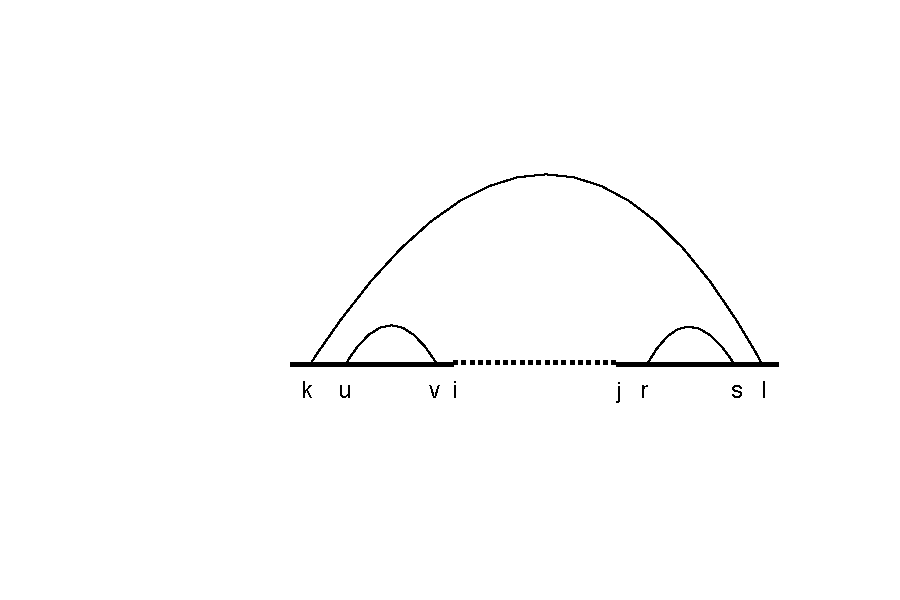
\includegraphics[width=0.8\textwidth]{lectures/160509/pix/RNAplex_Abb.pdf}
